\chapter{Introduction}

\section{Quantum Chromodynamics}

Early theoretical work in nuclear physics, after the discovery of the neutron, focused on establishing the theory of the strong force responsible for binding together protons and neutrons. The earliest model, that of Yukawa, relied on the exchange of a massive boson (the $\pi$ meson). Later experiments looking at harder interactions between nucleons showed that these processes could produce a large variety of hadrons, pointing to a much richer structure within protons and neutrons. Thus it became necessary to think beyond the model of the nuclear force (protons and neutrons exchanging pions), and instead look at the more fundamental strong force which gives rise to the structure and interaction of all hadrons. In the 1960s the quark model was developed and successfully explained the multiple observations of new hadrons being created in collider experiments by supposing that hadrons were not fundamental particles, but rather composed of quarks.

Quantum Chromodynamics (QCD) is the fundamental theory of the strong force and describes the interactions between quarks which is mediated by gluons. Quarks come in 6 flavors: up, down, strange, charm, bottom, and top. All quarks have a fractional electric charge (either $\pm \frac{1}{3}e$ or $\pm \frac{2}{3}e$). Quarks carry a color (red, green, or blue) and are bound by gluons into groups of three (baryons) or two (mesons). Baryons and mesons have no color, in baryons the three colors add up in a way that is color neutral while in mesons the one quark carries a color and the antiquark carries an anticolor. 

Deep inelastic scattering experiments at SLAC further probed the structure of nucleons and showed that they were composed of three spin-$1/2$ particles. These measurements confirmed the quark model and showed that quarks were real particles within hadrons. DIS experiments also suggested other peculiar and (at the time) unexpected behaviors in quarks. When bound quarks are probed at higher energy scales they behave as if they were free. In fact it is the case with quarks that with large momentum exchange the coupling between quarks and gluons is weak and we can treat QCD perturbatively. However as the energy scale decreases the coupling becomes stronger and perturbation theory no longer applies. This property of QCD is called asymptotic freedom and was discovered in 1973 by Gross, Wilczek, and Politzer for which they were awarded the Nobel Prize in 2004. Asymptotic freedom arises in QCD because it is a non-Abelian gauge theory. There is screening of the color charge of quarks by the vacuum, however there is also anti-screening from charged spin-1 gluons. The value of the coupling in QCD can be represented by the $\beta$ function, for QCD it can be shown that to lowest order $\beta(g)$ is propotional to $-(\frac{11}{2} - \frac{n}{3})$ where n is the number of quarks. For QCD, with 8 gluons and 3 colors, the anti-screening from the gluons overcomes the screening of the quarks and thus the theory is asyptotically free. Figure~\ref{fig:a_free} shows experimental estimates of $\alpha_S$ as well as the scale of the momentum exchange. Experimental results are in agreement with the predictions of asymptotic freedom. 

\begin{figure}[htbp]
\begin{center}
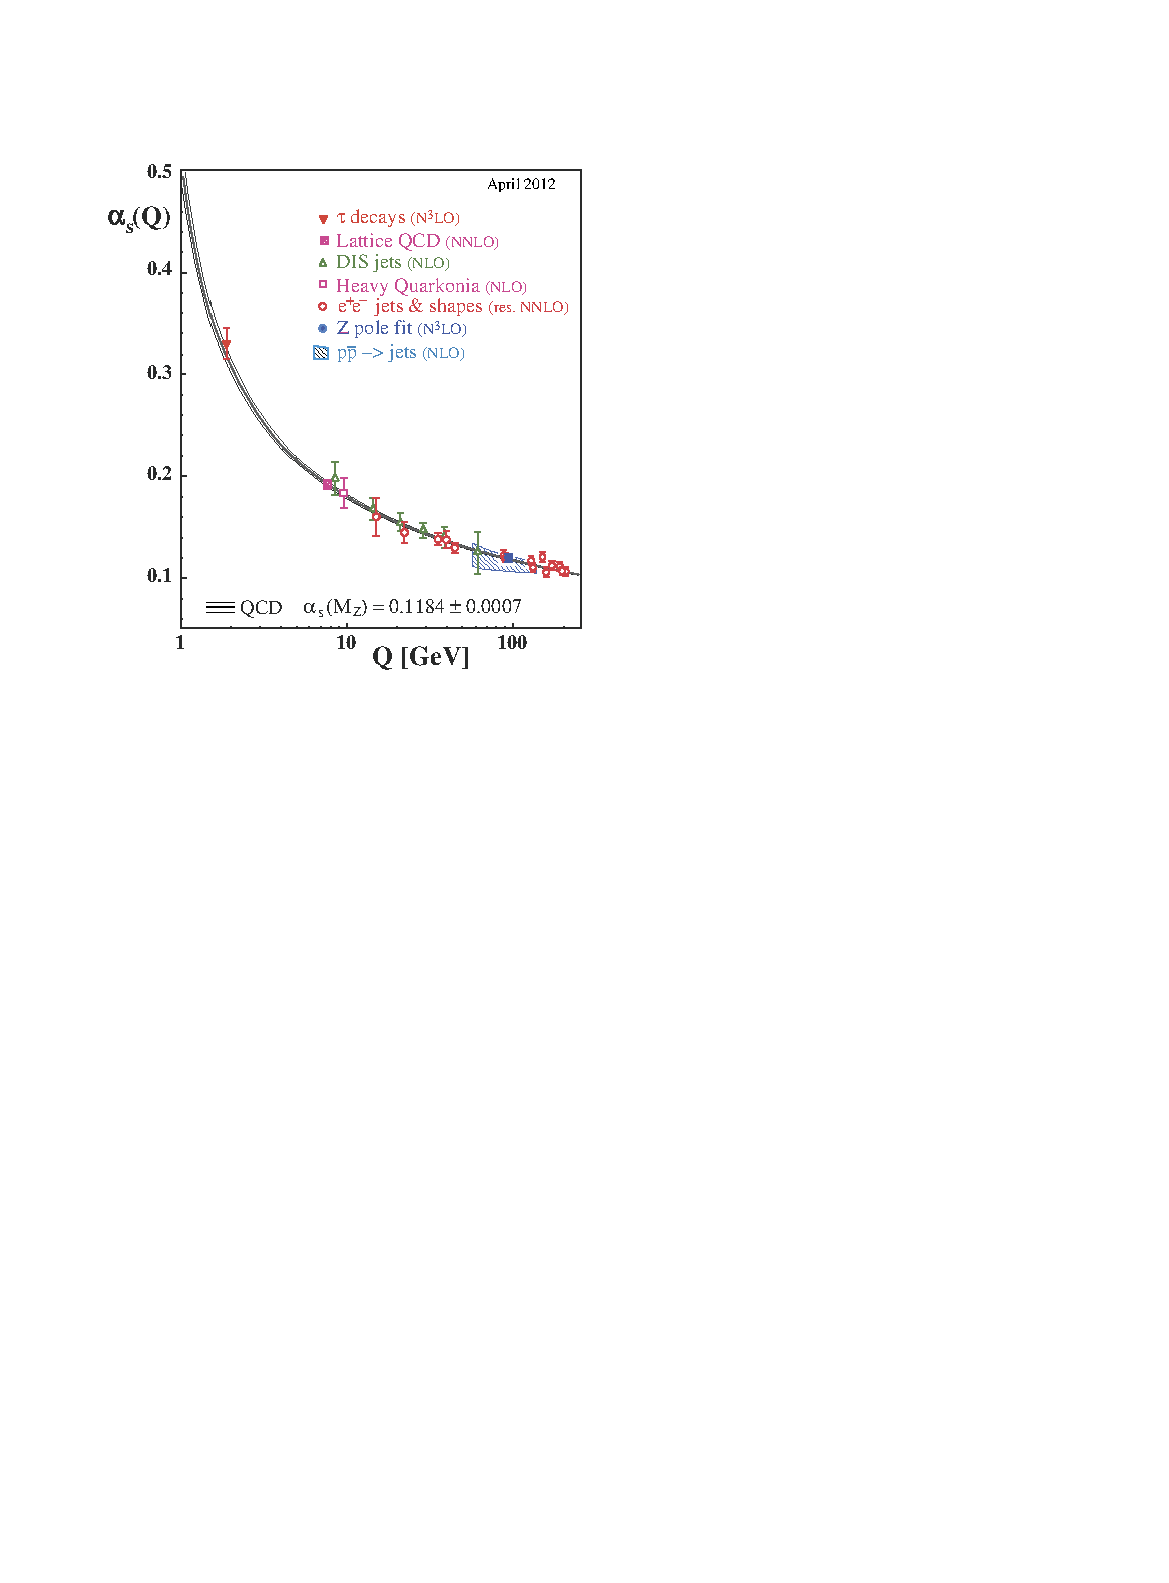
\includegraphics[scale=1.3]{Plots/Intro/asymp_free.pdf}
\end{center}
\caption[Asymptotic Freedom]{Several measurements of the strong coupling constant $\alpha_S$ showing how it varies with energy scale. Decreasing coupling strength as the interaction energy goes up is consistent with predictions of asymptotic freedom}
\label{fig:a_free}
\end{figure}

Within baryons and mesons quarks are bound in colorless states, and as explained above, at short distance scales the coupling between the quarks and gluons in weak and we can treat the interaction of quarks perturbatively. However, when we attempt to remove a quark from a hadron lattice QCD calculations show the potential increases linearly with distance. Eventually the energy put into this hypothetical system increases to a high enough point that a new quark anti-quark pair is created from the vacuum and we end up with two hadrons. This property of QCD, that quarks and gluons remain bound in colorless states, we refer to as confinement. 

Confinement and asymptotic freedom are two of the most interesting properties associated with QCD, and are responsible for many of the interesting phenomena within the strong interaction. As we dive deeper into QCD we will next explore the QCD phase diagram, and look for evidence of confinement being broken.  

\section{QCD Phase Diagram and Deconfinement}

At low temperatures lattice calculations show that quarks are confined within hadrons, we will now turn our attention to the properties of quark matter under more extreme conditions. Lattice calculations also predict a rich phase structure in QCD beyond just what we observe in low temperature hadronic matter. As we increase the temperature and density of nuclear matter it is predicted that quarks and gluons are deconfined from their hadronic states. We call this hot dense state of matter with strongly interacting free quarks and gluons the Quark Gluon Plasma (QGP). Conditions in the universe allowed for QGP to exist up until about $10^{-5}$s after the Big Bang. There is also the chance that colder deconfined matter could exist within neutron stars.

Figure~\ref{fig:qcd_phase} shows an illustration of the QCD phase diagram. Nuclear matter exists in the lower right part of the figure, inside nuclei the temperatures are low and the average net baryon number is high. The figure also shows the regions of the phase diagram which are accesible to various experiements which we will discuss further in upcoming sections. Also of note is that the phase transition from QGP to hadronic matter can be either a first order or second order phase transition and that there is postulated to be a critical point in the QCD phase diagram. The search for the QCD critical point is an area of active research, but is beyond the scope of this dissertation. 

\begin{figure}[htbp]
\begin{center}
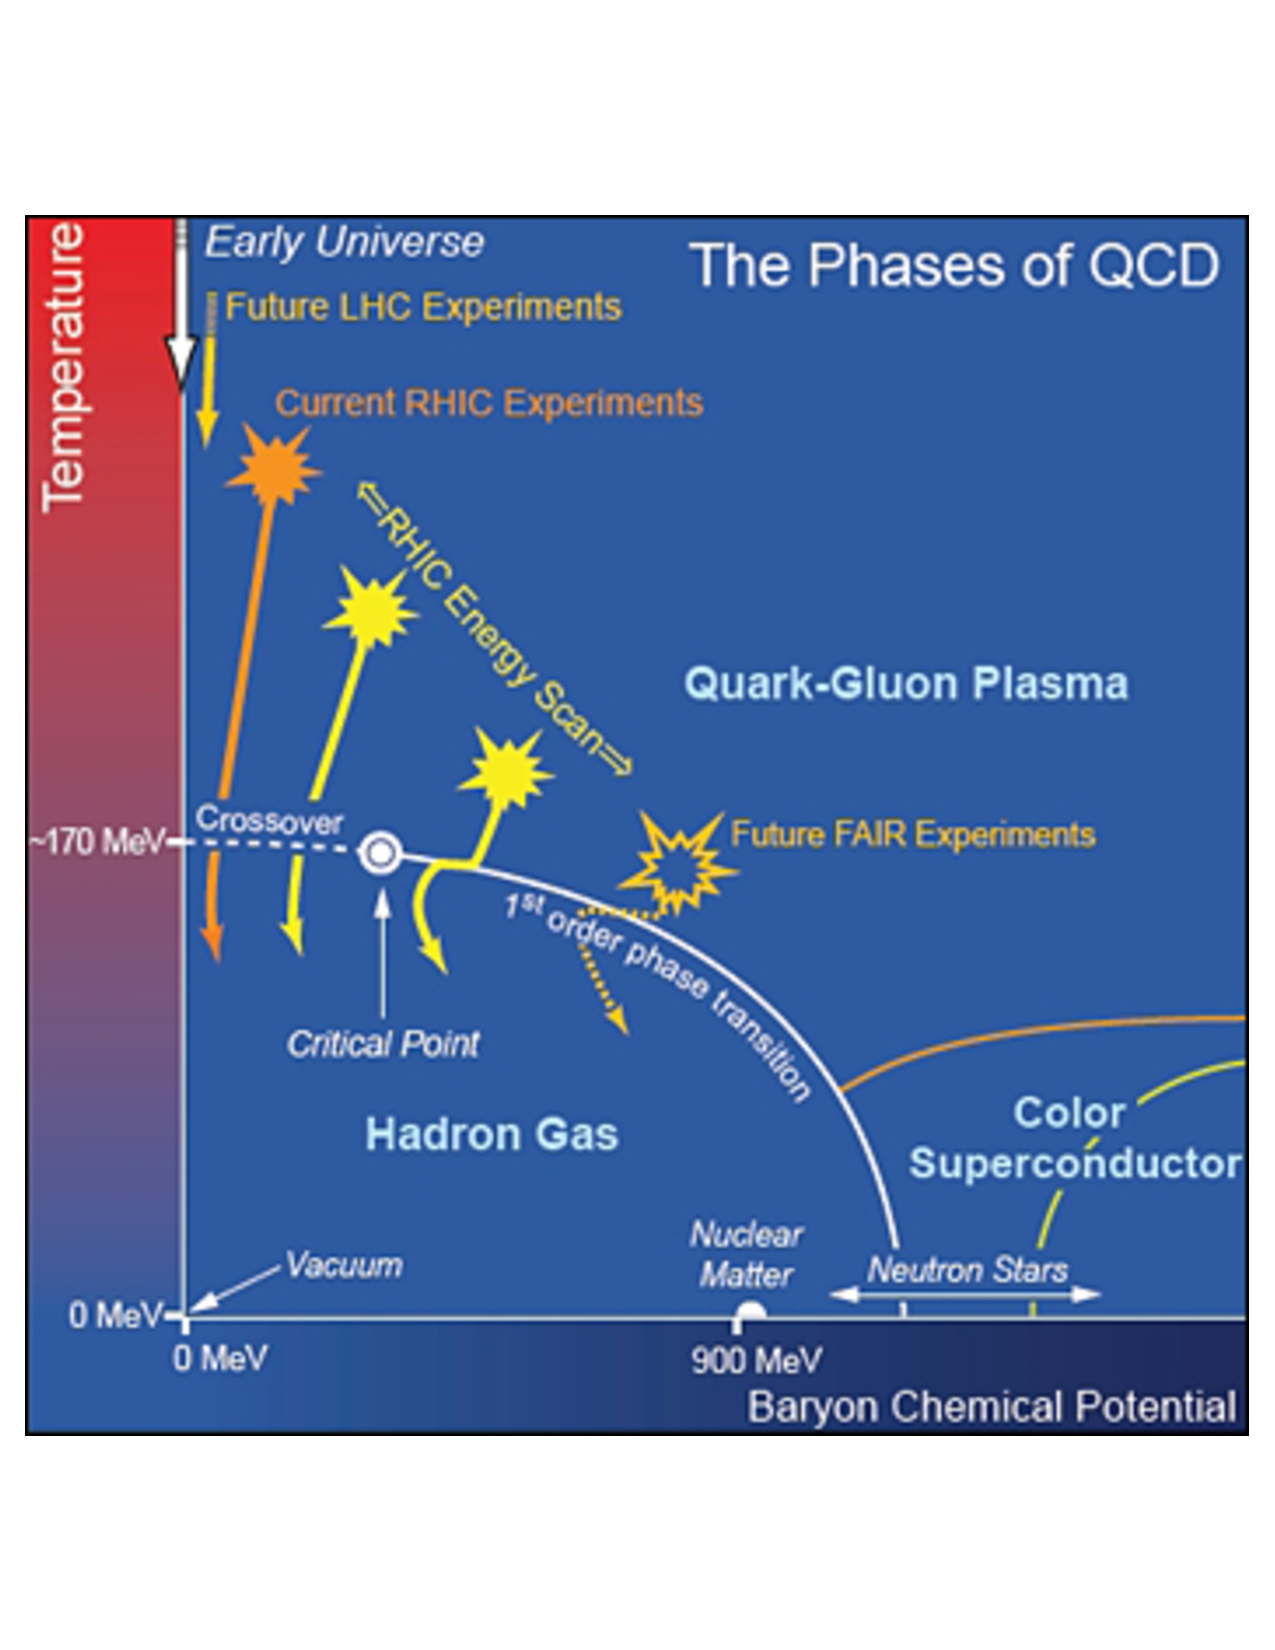
\includegraphics[scale=0.5]{Plots/Intro/qcd_phase.pdf}
\end{center}
\caption[QCD Phase Diagram]{Illustration of the QCD phase diagram showing the various regimes as well as the reach of current experiments.}
\label{fig:qcd_phase}
\end{figure}

The critical behavior in QCD can be seen in the bulk thermodynamic properties of QGP around the critical temperature $T_c$. Figure~\ref{fig:pressure} shows the quantity $p/T^4$ as a function of temperature for various quark flavor combinations. At the critical temperature there is a transition from hadronic to partonic degrees of freedom which is seen in the large jump in $p$. At high temperatures the medium behaves as an ideal gas. The increase in degrees of freedom is taken as evidence that the phase transition in QCD coicides with the onset of deconfinement.

\begin{figure}[htbp]
\begin{center}
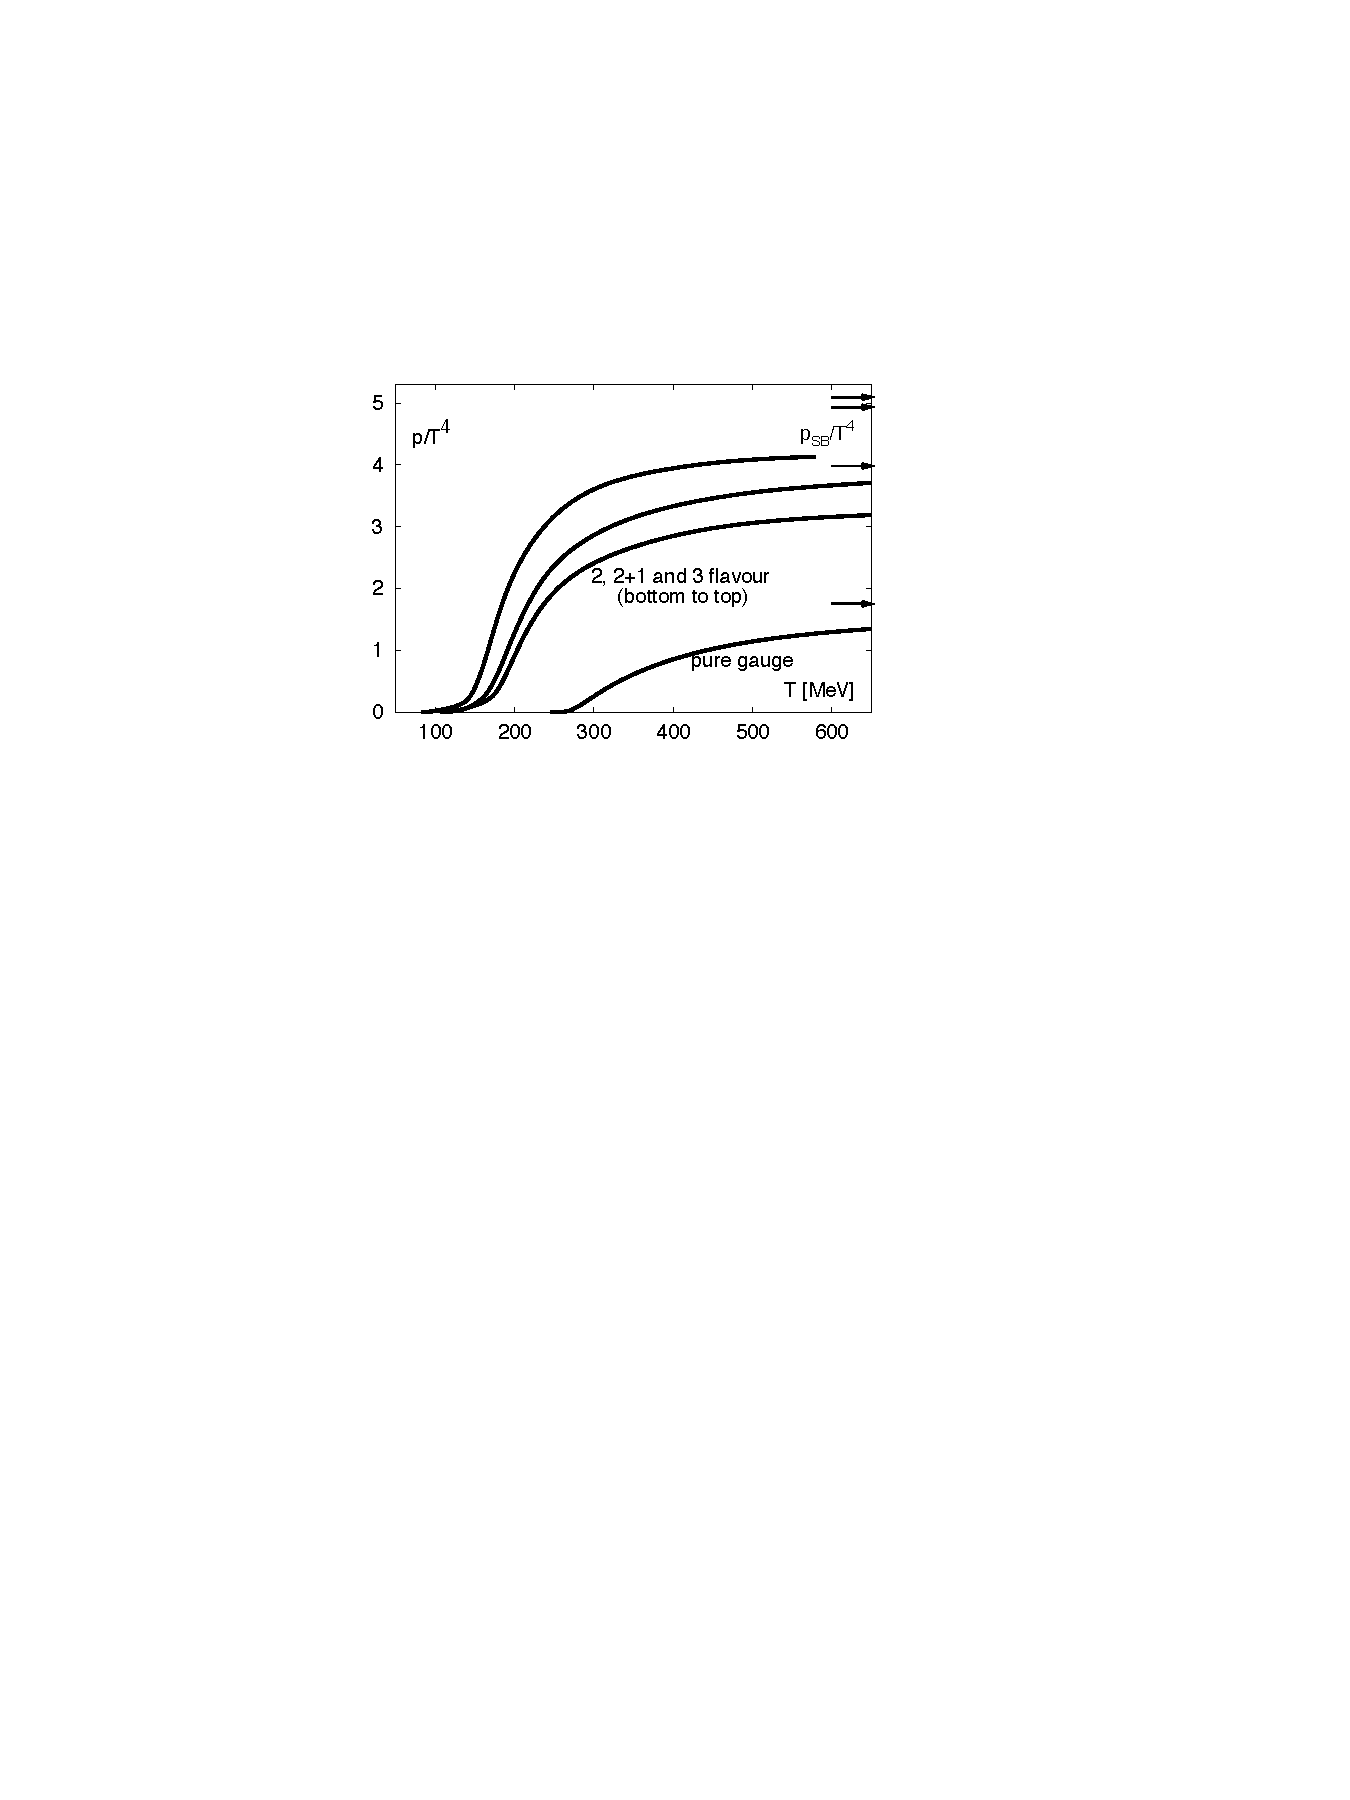
\includegraphics[scale=1.0]{Plots/Intro/pressure.pdf}
\end{center}
\caption[$p/T^4$ Calculations]{Calculations of $p/T^4$ in QCD for various numbers of quark flavors. Large jump near $T_c$ is the result of an increase in the number of degrees of freedom in the medium and is caused by the deconfinement of hadronic matter.}
\label{fig:pressure}
\end{figure}

\section{Experiments on QGP}

\subsection{Heavy Ion Collisions}

With the prediction that deconfined matter could exist at sufficiently high temperatures and densities, there was significant interest in creating these conditions experimentally. The idea was to collide the nuclei of heavy elements at relativistic speeds, at high enough energy, these collisions could recreate the conditions in the universe shortly after the big bang and cause hadronic matter to become deconfined. The first experiments looking for QGP were fixed target programs at the Alternating Gradient Synchrotron at Brookhaven and the Super Proton Synchrotron at CERN. Initial hints towards deconfinement were seen in these experiments. The WA97 and NA49 experiments observed large enhancement for strange baryons in Pb+Pb collsions which could be explained by a phase transition to a state with massless light quarks.

The early fixed target results pointed in the direction of QGP but were not conclusive proof of its existence. The next step for QGP research was to move to collider based experiments. In 2000 the Relativistic Heavy Ion Collider began operating with the capability to collide gold nuclei at 200 GeV center of mass energy per nucleon. Several years later the Large Hadron Collider began colliding lead nuclei at over 2 TeV center of mass energy. Key measurements have been made by the experiments at RHIC pointing towards the existence of a strongly interating deconfined phase of matter. We will now discuss some of these results which include: thermal production of light hadrons, elliptic flow of particles, and suppression of high $p_T$ particles and jets in central collisions. We will then look in particular at the measurements made in the heavy flavor sector (charm and bottom quarks) and motivate future observations there.

\subsection{Hadron Yields}

To look for signs of the QCD phase transition and the QGP, we want to study central collisions of heavy ions. In heavy ion collisions the two nuclei are offset from each other by some impact parameter, and thus their region of overlap is an ellipsoid. We refer to the degree of overlap between the nuclei as the centrality and typically describe events by which percentile of centrality they fall into e.g. 10\%-20\% central (lower number corresponds to more central). The most central collisions have the largest fireballs and thus the most favorable conditions for producing QGP. 

One measurement to perform in heavy ion collisions is to measure the yields of hadrons from central collisions and compare them to thermal statistical models to extract the temperature and baryon chemical potential. Figure~\ref{hadron_yields} shows the yields for several hadrons as measured by the experiments at RHIC along with the yields as determined by the fits to a thermal statistical model. From this the temperature at chemical freeze-out (the point in the collision at which particle flavors are fixed) and is calculated to be 164 MeV.

\begin{figure}[htbp]
\begin{center}
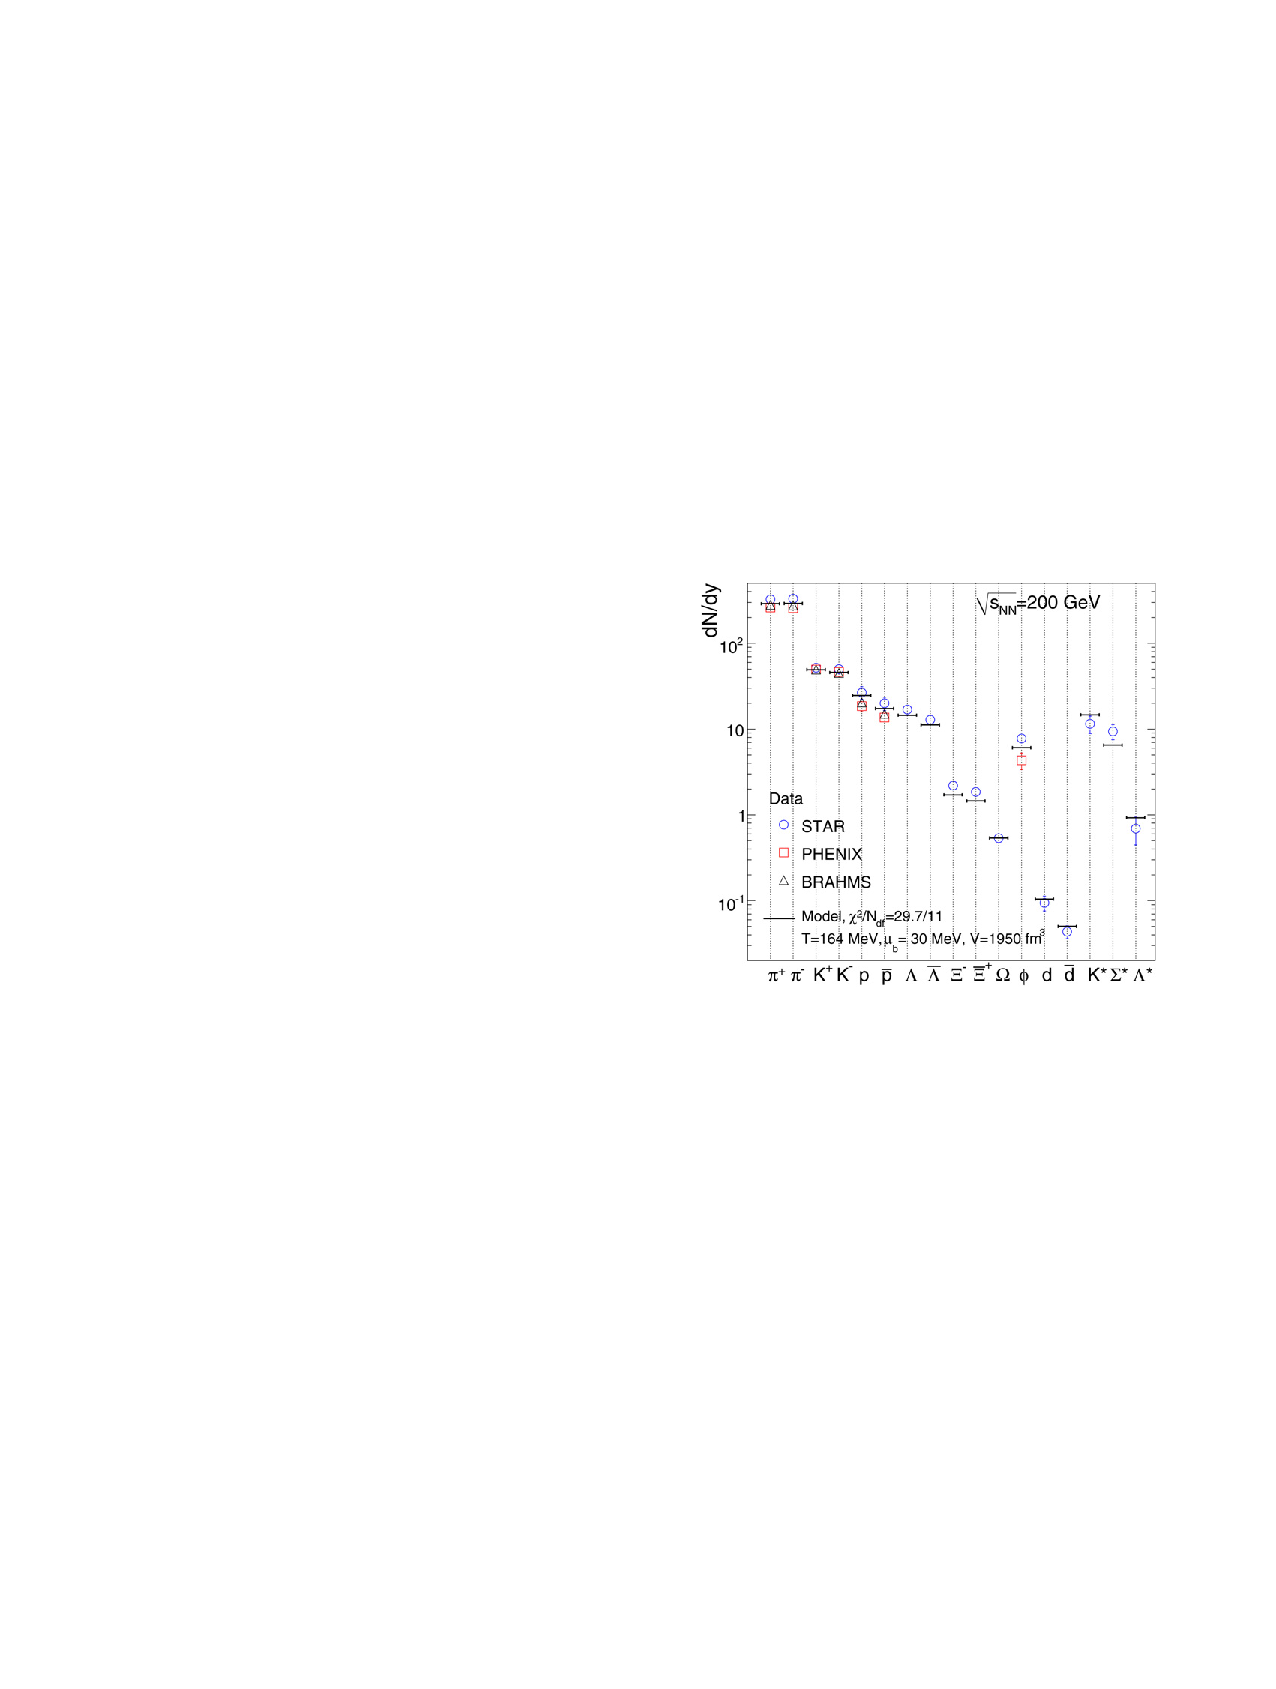
\includegraphics[scale=1.2]{Plots/Intro/had_yields.pdf}
\end{center}
\caption[Hadron Yields]{Yields for various hadrons in central collisions at RHIC energies compared to calculations from themal statistical models.}
\label{fig:hadron_yields}
\end{figure}

Comparisons can be made across several experiements with different collision energies to look for evidence of a phase transition, this is shown in Figure~\ref{fig:T_mu}. This shows the T and $\mu_B$ extracted from the thermal statistical model fits as a function of the collision energy. The lower points come from the fixed target programs at the AGS and SPS while the highest data point corresponds to RHIC energies. The flattening of the temperature at chemical freeze-out around T $\approx$ 160 MeV as energy increases is suggestive of a QCD phase boundary.

\begin{figure}[htbp]
\begin{center}
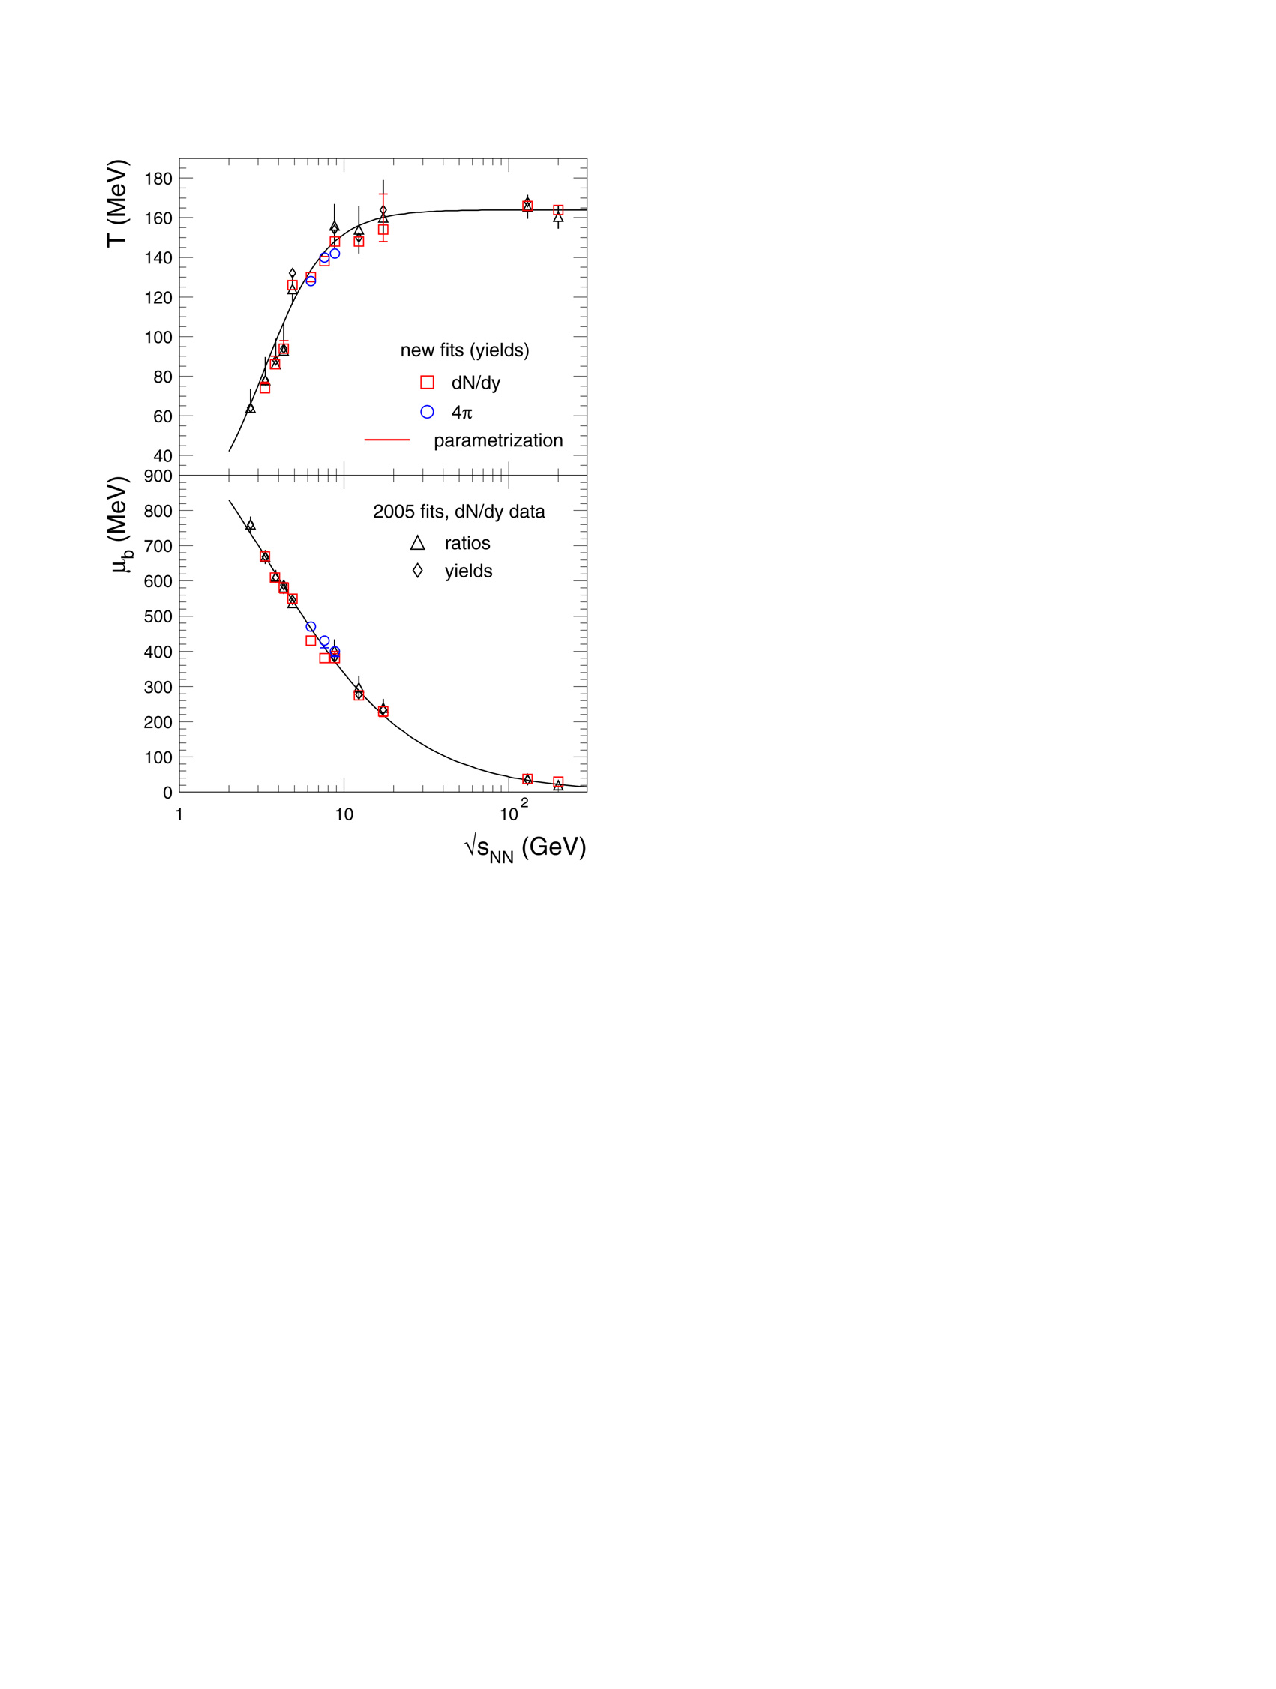
\includegraphics[scale=1.3]{Plots/Intro/freezeout.pdf}
\end{center}
\caption[Freeze-out T and $\mu_B$]{Temperature and baryon chemical potential extracted from thermal statistical model as a function of collision energy.}
\label{fig:T_mu}
\end{figure}

\subsection{Elliptic Flow}

In heavy ion collisions the nuclei do not exactly overlap, instead leaving an ellipsoidal region where temperatures and densities are high enough to create quark gluon plasma. This ellipsoidal overlap region creates an initial position space anisotropy which creates a pressure gradient along the fireball which manifests itself as an momentum dependent azimuthal anisotropy in the final state, which we call elliptic flow. More formally, the distribution of particles as a function of azimuthal angle can be written out as a Fourier expansion:

\begin{equation}\label{eq:v2def}
E\frac{d^3N}{d^3p} = \frac{1}{2\pi}\frac{d^2N}{p_Tdp_Tdy}[1 + \sum_{n=1}^{\infty}2 v_n \cos{n(\phi - \Psi_r)}]
\end{equation}

Where $\Psi_r$ is the angle of the reaction plane, which for our purposes can be thought of as the plane perpendicular to the major axis of the ellipsoid. The elliptic flow is the coefficient of the second term of this expansion, $v_2$. In Au+Au collisions at RHIC $v_2$ is large for light hadrons and consistent with hydrodynamic models at low $p_T$ ($\leq 2$ GeV), at higher $p_T$ the contribution of jets to $v_2$ needs to be considered. These measurements of $v_2$ point to a high degree of thermalization in collisions at RHIC energies and the mass dependence of $v_2$ indicates a collective flow of the medium.

%section and figure for NCQ scaling

\subsection{$R_{AA}$ and Jet Suppression}

\section{Heavy Flavor Probes}

\section{Two Particle Correlations}
